\documentclass[aspectratio=1610]{beamer}

\usepackage{lmodern}			% Usa a fonte Latin Modern			
\usepackage[T1]{fontenc}		% Selecao de codigos de fonte.
\usepackage[utf8]{inputenc}		% Codificacao do documento (conversão automática dos acentos)
\usepackage{lastpage}			% Usado pela Ficha catalográfica
\usepackage{indentfirst}		% Indenta o primeiro parágrafo de cada seção.
\usepackage{color}				% Controle das cores
\usepackage{graphicx}			% Inclusão de gráficos
\usepackage{microtype} 			% para melhorias de justificação
%\usepackage{helvet}
%\usepackage{sfmath}
\usepackage{tcolorbox}
\usepackage{tikz}
\usetikzlibrary{shapes,arrows,automata,calc}
\usepackage{pgfplots}
\pgfplotsset{compat=newest}
\usepgfplotslibrary{groupplots}
\usepgfplotslibrary{dateplot}
\usepackage{subfiles}
\usepackage{subcaption}
\usepackage{siunitx}
\usepackage[olditem,oldenum]{paralist}
\usepackage{pdfpages}
\usepackage{amsmath}
\usepackage{amssymb}
\usepackage{mathtools}
\usepackage[ruled]{algorithm2e}
\usepackage{multicol}
\usepackage{rotating}
\usepackage{pdflscape}
\usepackage{everypage}
\usepackage[font={small,sf, singlespacing}, margin=2cm]{caption}
\usepackage{svg}
\usepackage[style=abnt,language=english,pretty]{biblatex}
\usepackage{morewrites}
\usepackage[acronym,acronymlists={symbol},shortcuts]{glossaries}
\usepackage{cleveref}

% Citações padrão ABNT.
% Uncomment to use bibtex 
%\usepackage[alf]{abntex2cite}	

% Uncomment to use biblatex
\addbibresource{references/references.bib}        % Seus arquivos de
\addbibresource{references/numeric/numeric.bib}        % Seus arquivos de
\addbibresource{references/turbine/turbine.bib}        % Seus arquivos de
%\addbibresource{outroarquivo.bib}   % bibliografia vão aqui

%Acronyms and list of symbols
\newglossary[slg]{symbol}{sot}{sym}{List of Symbols}
\makeglossaries
\renewcommand{\acronymname}{List of abbreviations and acronyms}

 % Use long (short) acronym style:
\setacronymstyle{long-short}

%Preamble inputs
\newcommand{\stagdensratio}[1]{\left( 1+\frac{\gamma-1}{2}M_{#1}^2\right)^\frac{1}{\gamma-1}}
\newcommand{\MFP}[1]{\frac{\dot{m}\sqrt{RT_{0#1}}}{A_{#1} P_{0#1} \sqrt{\gamma}}}
\newcommand{\MFPalt}[1]{\frac{\dot{m}}{A_{#1} \rho_{0#1} a_{0#1}}}
\newcommand{\pr}[2]{\frac{P_{#1}}{P_{#2}}}
\newcommand{\volume}{{\ooalign{\hfil$V$\hfil\cr\kern0.08em--\hfil\cr}}}

\newacronym[type=symbol]{N}{\ensuremath{N}}{shaft rotational speed}
\newacronym[type=symbol]{T0}{\ensuremath{T_0}}{ambient temperature}
\newacronym[type=symbol]{P0}{\ensuremath{P_0}}{ambient pressure}
\newacronym[type=symbol]{delta}{\ensuremath{\delta}}{$\text{inlet pressure}/\text{\acs{ISA} pressure at sea level}$}
\newacronym[type=symbol]{theta}{\ensuremath{\theta}}{$\text{inlet temperature}/\text{\acs{ISA}temperature at sea level}$}

% Euler equation
\newacronym[type=symbol]{torque}{\ensuremath{\tau}}{torque}
\newacronym[type=symbol]{power}{\ensuremath{\text{power}}}{power}
\newacronym[type=symbol]{U}{\ensuremath{U}}{rotor speed}
\newacronym[type=symbol]{r}{\ensuremath{r}}{rotor radius}
\newacronym[type=symbol]{V}{\ensuremath{V}}{absolute velocity}
\newacronym[type=symbol]{h}{\ensuremath{h}}{specific enthalpy}
\newacronym[type=symbol]{omega}{\ensuremath{\omega}}{angular speed}
\newacronym[type=symbol]{beta}{\ensuremath{\beta}}{specific enthalpy}
\newacronym[type=symbol]{load_coef}{\ensuremath{\psi}}{load coefficient $\frac{\Delta h}{U_2^2}$}
\newacronym[type=symbol]{flow_coef}{\ensuremath{\phi}}{flow coefficient $\frac{{\dot{m}}}{U\rho A}$}
\newacronym[type=symbol]{impeller_distortion_factor}{\ensuremath{\lambda}}{impeller distortion factor}
\newacronym[type=symbol]{slip_factor}{\ensuremath{\sigma}}{slip factor}
\newacronym[type=symbol]{MFP}{\text{MFP}}{mass flow parameter $\frac{\dot{m}\sqrt{RT_{01}}}{A_1 P_{01} \sqrt{\gamma}}$}
\newacronym[type=symbol]{M0rotor}{\ensuremath{M_{0\text{impeller}}}} {impeller stagnation mach number $\frac{U_2}{\sqrt{\gamma R T_{01}}}$}
\newacronym[type=symbol]{Re}{\text{Re}} {Reynolds number}
\newacronym[type=symbol]{gam}{\ensuremath{\gamma}} {specific heat ratio $\tfrac{c_p}{c_v}$}


\newacronym{FADEC}{FADEC}{Full Authority Digital Engine Controler}
\newacronym{EGT}{EGT}{Exhaust Gas Temperature}
\newacronym{ECU}{ECU}{Engine Control Unit}
\newacronym{CAD}{CAD}{Computer Assisted Design}
\newacronym{TLA}{TLA}{Thrust Level Angle}
\newacronym{T-MATS}{T-MATS}{Toolbox for the Modeling and Analysis of Thermodynamic Systems}
\newacronym{GSP}{GSP}{Gas turbine Simulation Program}
\newacronym{ALFALAB}{ALFALAB}{Aerospace Laboratory and Fabrication}
\newacronym{ISA}{ISA}{International Standard Atmosphere}
\newacronym{SL}{SL}{sea level}
\newacronym{IGV}{IGV}{inlet guide vanes}
\newacronym{ODE}{ODE}{ordinary differential equation}
\newacronym{DAE}{DAE}{differential-algebraic equations}


%% Uncomment this to disable source in figures
%\renewcommand{\source}[1]{}

%% Configurações de aparência do PDF final

% alterando o aspecto da cor azul
\definecolor{blue}{RGB}{41,5,195}


\usepackage[brazil]{babel}
\usepackage{multimedia}

\usetheme[%sectionpage=none,
          %numbering=fraction,
          progressbar=head]{metropolis}
\setbeamercolor{background canvas}{bg=white}

\title{Simulação de motores a jato}
\author{Bernardo Bahia Monteiro}
\institute{Universidade Federal de Minas Gerais}
\date{26 de junho de 2019}

\begin{document}
\maketitle

\begin{frame}
\frametitle{Agenda}
\tableofcontents
\end{frame}

\clearpage

\section{Introdução} %Motivação
\begin{frame}[t]
\frametitle{O motor a jato}
\centering

%\the\textwidth

\only<1>{\includesvg{fig/engine_schematic_presentation1}}
\only<2>{\includesvg{fig/engine_schematic_presentation2}}

\end{frame}
\note{
Este é um desenho esquemático do motor com o qual vamos trabalhar. Trata-se de um motor turbojato com compressor centrífugo e turbina axial.

A numeração das estações dentro do motor segue o padrão da indústria:
a estação 2 é a entrada do compressor; 3 saída do compressor, 4 entrada da turbina; 5 saída da turbina; e 9 saída do bocal.
}

\begin{frame}
\frametitle{Por que simular um motor a jato?}
Verificar o projeto fora do ponto de projeto

\vspace{1em}

Desenvolver o sistema de controle. Queremos operar perto da
    \begin{itemize}
        \item velocidade máxima do eixo
        \item temperatura máxima da turbina
        \item limite de estabilidade do compressor
        \item limite de estabilidade da queima
        \item região de máxima eficiência
    \end{itemize}
\end{frame}

%\subsection{Estabilidade de um motor a jato}
\begin{frame}
    \frametitle{Extinção de chama (blowout)}
        \begin{center}
        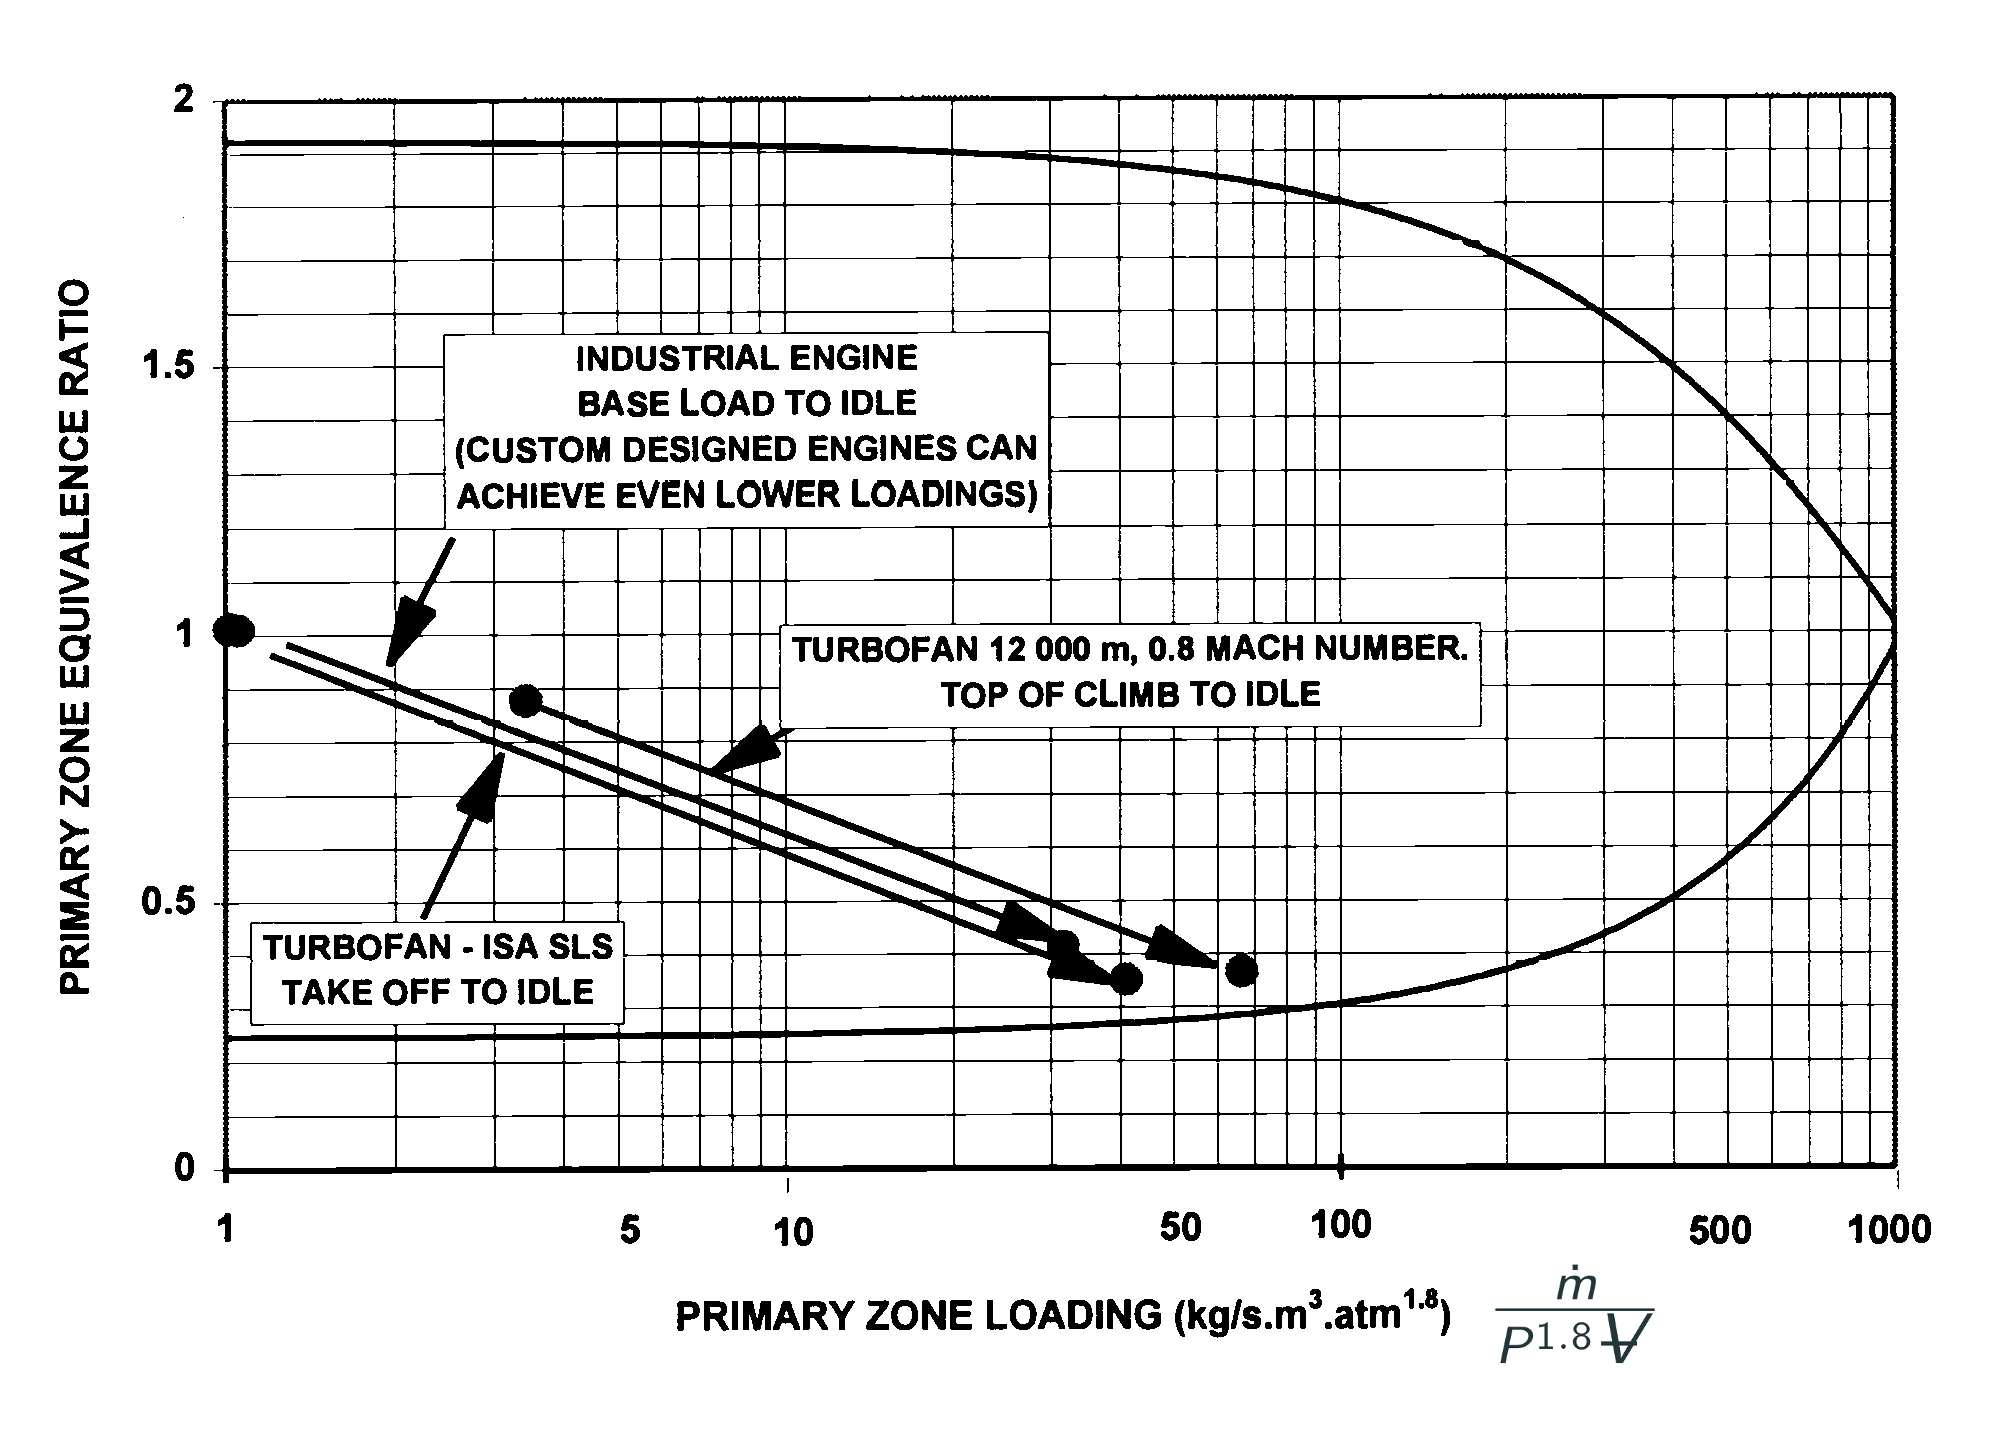
\includegraphics[height=3in]{fig/combustion_stability}
        \end{center}
        \vspace{-1em}
        {\scriptsize\cite{walsh2004gas}}
\end{frame}

{
\setbeamercolor{background canvas}{bg=black}
\begin{frame}
    \frametitle{Purga do compressor}
    \centering
    \pgfdeclareimage[width=4in]{surgethumb}{fig/surge_thumb}
    \movie[width=4in, height=3in]{\pgfuseimage{surgethumb}}{../fig/surge.mp4}
\end{frame}
}

\begin{frame}
    \frametitle{Como simular um motor a jato?}
     Comportamento de cada componente
            \begin{itemize}
                \item relação entre $\dot{m}$, $\omega$, e as razões de $P$ e  $T$
            \end{itemize}
            \vspace{1em}
     Casamento dos componentes
            \begin{itemize}
                \item equações de conservação
            \end{itemize}

\end{frame}


\begin{frame}
    \frametitle{Números adimensionais}
    
    \begin{columns}
        \column{0.5\textwidth}
        \begin{align*}
            M_b &= \frac{\omega r}{a_{0i}} \\[2em]
            \acs{MFP}_n &= \MFP{n} = \MFPalt{n} 
        \end{align*}
        
        \column{0.5\textwidth}
        \only<2>{\centering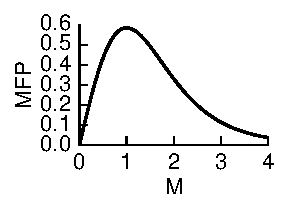
\includegraphics{fig/mfp_fig}}
    \end{columns}
\end{frame}

\section{Modelo dos componentes} %compressor e turbina
\begin{frame}
    \frametitle{Mapa do compressor}
    \centering
    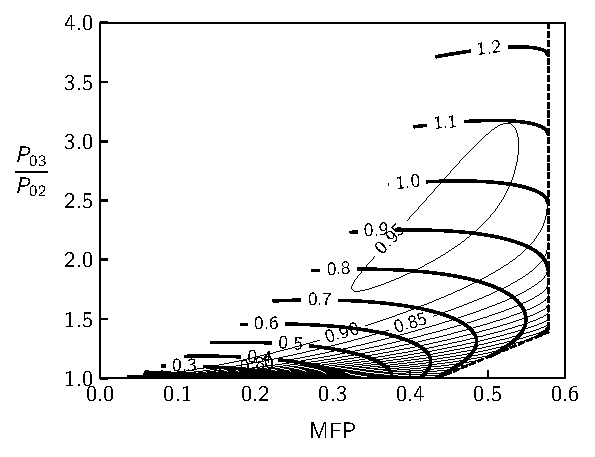
\includegraphics{fig/compressor_map}
\end{frame}

\note{Mas como esse mapa é gerado?}
\begin{frame}
\frametitle{Modelo do compressor}

\begin{block}{Variáveis}
    \[
        \acs{MFP}_2, \quad \acs{MFP}_3, \quad M_{bc}, \quad \tr{03}{02}, \quad \pr{03}{02}
    \]
\end{block}

\vfill
    
\begin{block}{Equações}
\begin{itemize}
    \item Conservação do momento angular (equação de Euler)
    \item Conservação de massa
    \item Modelo de perdas
\end{itemize}
\end{block}
    \vfill
    \textbf{Graus de liberdade:} 2 
\end{frame}


\note{O fluxo de massa na entrada e na saída determina a velocidade do fluído. 
Em conjunto com  a rotação, os angulos do escoamento são determinados. 
a equação de conservação do momento angular, chamada equação de Euler, 
liga esses ângulos ao aumento de entalpia ideal que ocorre no compressor.
finalmente o modelo de perdas transforma o aumento de entalpia ideal em um aumento de entalpia real, que é usado para calcular o aumento de temperatura e um aumento de entalpia do processo isentrópico equivalente, que é usado para calcular o aumento de pressão no compressor.
}

\begin{frame}
    \frametitle{Modelo de perdas do compressor}
    \begin{columns}
        \column{0.5\textwidth}
        \begin{itemize}
            \item Perda por incidência
            \item Perda por carga na pá
            \item Perda por fricção
        \end{itemize}
        \column{0.5\textwidth}

        \only<2>{\includesvg{fig/incidence_loss1}}
        \only<3>{\includesvg{fig/incidence_loss2}}
        \only<4>{\includesvg{fig/incidence_loss3}}
    \end{columns}

\end{frame}

\begin{frame}
    \frametitle{Mapa da turbina}
    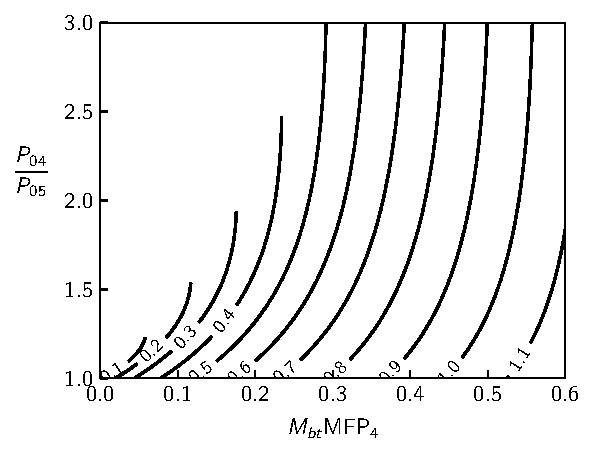
\includegraphics{fig/turbine_map_typical}
\end{frame}

\note{Mas como esse mapa é gerado?}
\begin{frame}
\frametitle{Modelo da turbina}

\begin{block}{Variáveis}
    \[
        \acs{MFP}_4, \quad \acs{MFP}_5, \quad M_{bt}, \quad \tr{05}{04}, \quad \pr{05}{04}
    \]
\end{block}

\vfill
    
\begin{block}{Equações}
\begin{itemize}
    \item Conservação do momento angular (equação de Euler)
    \item Conservação de massa
    \item Modelo de perdas
\end{itemize}
\end{block}
    \vfill
    \textbf{Graus de liberdade:} 2 
\end{frame}

\section{Modelo do motor} % dinâmico e estático
\begin{frame}
    \frametitle{Modelo estático do motor}

    \begin{block}{Variáveis}
        \begin{tabular}{ll}
            Compressor & $ \acs{MFP}_2, \quad \acs{MFP}_3, \quad M_{bc}, \quad \tr{03}{02}, \quad \pr{03}{02}$ \\
            Turbina    & $ \acs{MFP}_4, \quad \acs{MFP}_5, \quad M_{bt}, \quad \tr{05}{04}, \quad \pr{05}{04}$ \\
            Adicionais & $\dot{m}_f, \quad T_{04}$ \\
        \end{tabular}
    \end{block}
    \vfill
    \begin{block}{Equações}
    \begin{itemize}
        \item Modelo do compressor (3 eq.) e da turbina (3 eq.)
        \item Conservação de energia no eixo
        \item Conservação de massa na câmara de combustão
        \item Adição de energia pela queima
        \item Expansão isentrópica no bocal 
    \end{itemize}
    \end{block}

    \textbf{Graus de liberdade:} 1 
\end{frame}

\begin{frame}
    \frametitle{Modelo dinâmico do motor}

    \begin{block}{Variáveis}
        \begin{tabular}{ll}
            Compressor & $ \acs{MFP}_2, \quad \acs{MFP}_3, \quad M_{bc}, \quad \tr{03}{02}, \quad \pr{03}{02}$ \\
            Turbina    & $ \acs{MFP}_4, \quad \acs{MFP}_5, \quad M_{bt}, \quad \tr{05}{04}, \quad \pr{05}{04}$ \\
            Adicionais & $ t, \quad \dot{m}_f, \quad T_{04}, \quad P_{04}, \quad\rho_{04}$ \\
        \end{tabular}
    \end{block}
    \vfill
    \begin{block}{Equações}
    \begin{compactitem}
        \item Modelo do compressor (3 eq.) e da turbina (3 eq.)
        \item Rotação do compressor igual a da turbina
        \item Conservação de energia no eixo permitindo aceleração
        \item Conservação de massa no queimador (densidade variável)
        \item Conservação de quantidade de movimento no queimador
        \item Adição de energia pela queima
        \item Expansão isentrópica no bocal
        \item Equação do gás ideal no queimador
    \end{compactitem}
    \end{block}

    \textbf{Graus de liberdade:} 2 
    \hspace{6em}
    \textbf{Estados:} $\omega$, $\dot{m}$, $\rho_{04}$
\end{frame}

\section{Aspectos numéricos}
\begin{frame}
    \frametitle{Tipos de sistemas não lineares implícitos}
    \begin{columns}
        \column{0.3\textwidth}
        \only<1->{\[ f(x) = 0 \]}
        \column{0.3\textwidth}
        \only<2->{\[ f(t, x, \dot{x}) = 0 \]}
        \column{0.3\textwidth}
        \only<4->{\[ f(t, x, \dot{x}, \nabla x) = 0 \]}

    \end{columns}
        \vspace{1em}
        \makebox[0pt][t]{%
  \raisebox{-\totalheight}[0pt][0pt]{
        \hspace{0.33\textwidth}
        \only<3>{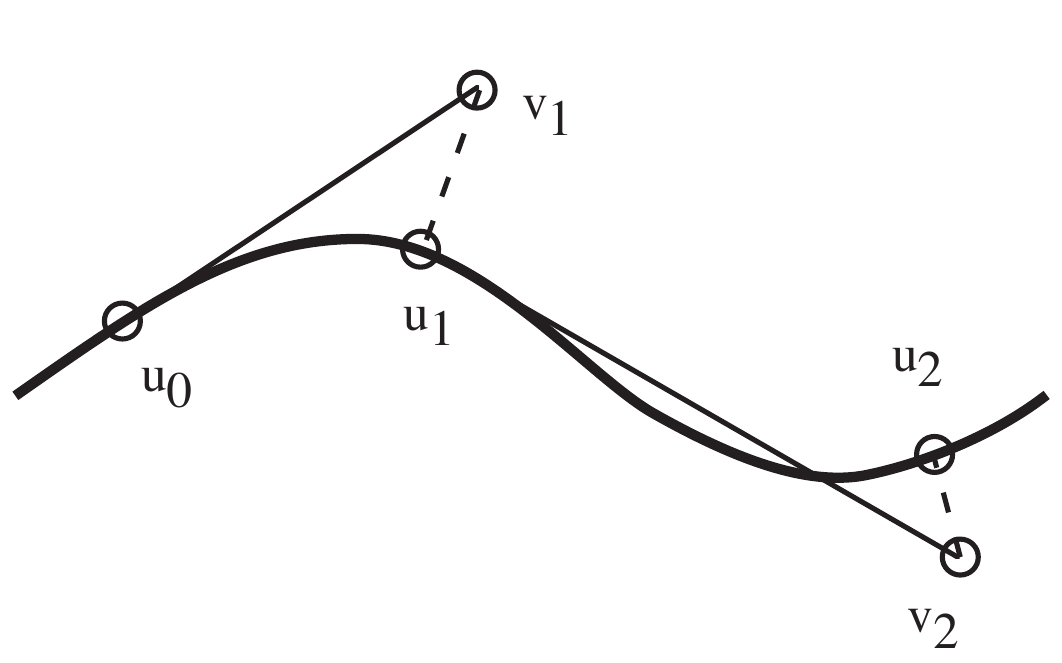
\includegraphics[width=0.3\textwidth]{fig/path_following.png}
        \scriptsize\cite{Allgower1997}
        }
        }}
\end{frame}

\begin{frame}
    \frametitle{Sistemas não lineares implícitos}
    \centering
    \begin{tabular}{lccccc}
        \toprule
        modelo & variáveis & \multicolumn{3}{c}{equações} & DOF \\ 
               &              & alg. & ODE & PDE          &     \\\midrule
        compressor       & 5  & 3    & -   & -    & 2 \\
        turbina          & 5  & 3    & -   & -    & 2 \\
        motor (estático) & 12 & 11   & -   & -    & 1 \\
        motor (dinâmico) & 15 & 10   & 3   & -    & 2 \\
        purga (estática) & 12 & 10   & -   & 1    & 1 \\
        \bottomrule
    \end{tabular}
\end{frame}        


\section{Resultados}

\begin{frame}
\frametitle{Linha de operação}
\makebox[\linewidth]{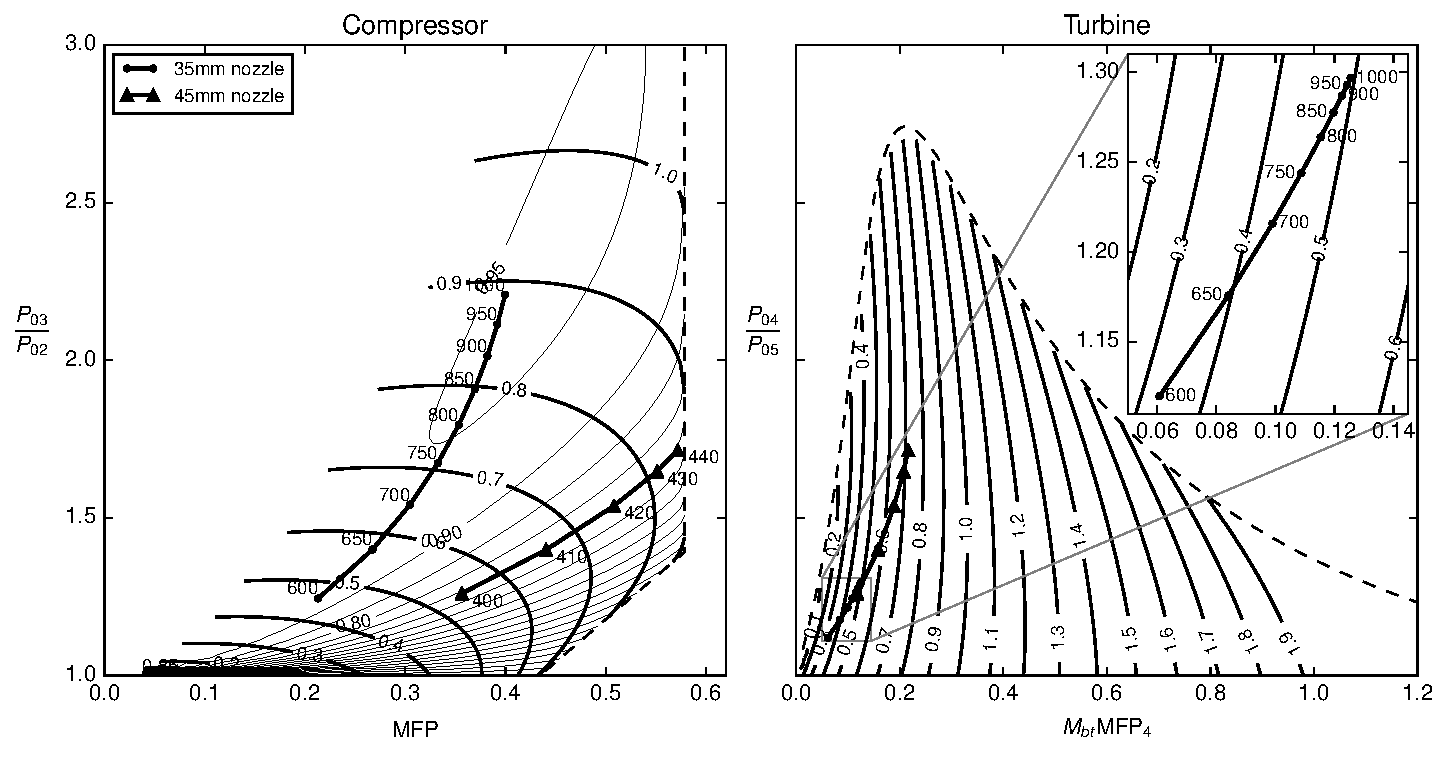
\includegraphics[width=\paperwidth, height=0.95\textheight, keepaspectratio]{fig/wline.pdf}}
\end{frame}

\begin{frame}
\frametitle{Ponto de operação $@ T_4=1000\si{K}$}
\centering
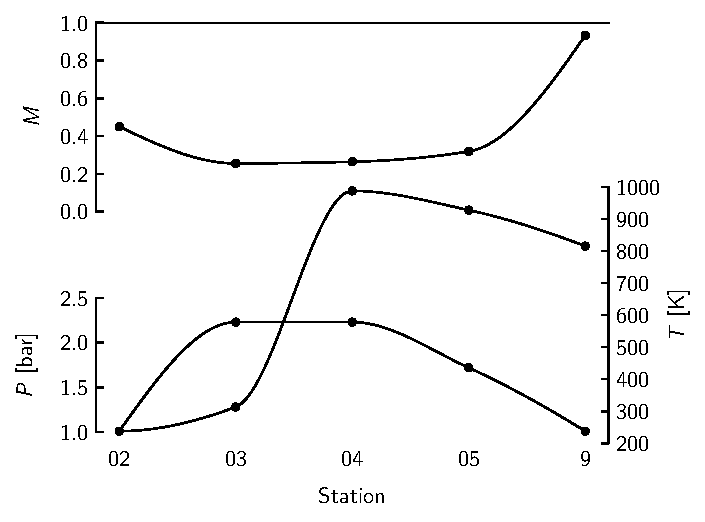
\includegraphics[width=\paperwidth, height=0.95\textheight, keepaspectratio]{fig/stations1000K}
\end{frame}

\begin{frame}
    \frametitle{Comparação com dados experimentais}
    \centering
    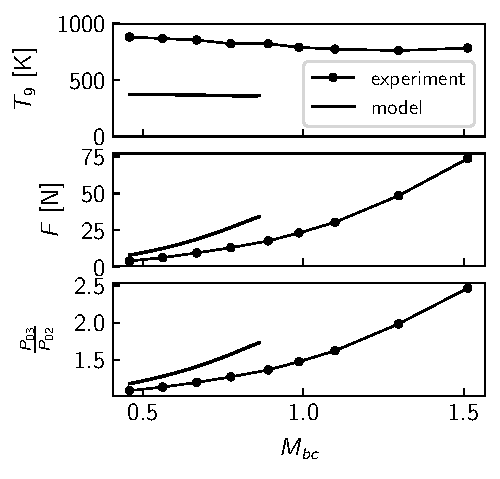
\includegraphics[width=\paperwidth, height=0.95\textheight, keepaspectratio]{fig/experimental_presentation}
\end{frame}

\section{Conclusão}
\begin{frame}
    \frametitle{Conclusão}
    \begin{itemize}
        \item É possível simular realisticamente um motor a jato
        \item Os modelos são expressos naturalmente como sistemas não lineares implícitos
        \item Esses sistemas devem ser resolvidos por métodos numéricos robustos
    \end{itemize}
    \vfill
    \begin{block}{Trabalhos futuros}
        \begin{itemize}
            \item Melhorar modelo de perdas
            \item Implementar modelo de purga
            \item Validadar com dados experimentais
        \end{itemize}
    \end{block}
\end{frame}

\begin{frame}
    \huge Obrigado!
\end{frame}


\end{document}
